\section{\libvmem: a userspace allocator with a broker}
\label{sec:libvmem}

\subsection{Motivation}
\label{sec:lv-motivation}

\Cref{sec:tr-flaw} showed that we cannot move memory under a running kernel
from userspace. A transparent design never learns when a buffer is idle, so
it has no safe moment to move it. We therefore give up transparency. The
application calls our allocator directly, and it tells us when a buffer is
idle.

The two standard options do not fit several processes that share one GPU.
With \code{cudaMalloc}, the next allocation fails once VRAM is full. With
UVM, every process keeps running, but the driver decides for the whole device
which pages stay in VRAM, and the application can only give advisory hints.
We want a middle ground with four properties:

\begin{itemize}
  \item each process keeps fast device memory while there is room;
  \item a process that finds the device full gets host memory and runs
    slower, instead of failing;
  \item memory moves only when the application says a buffer is idle;
  \item one component sees the memory use of every process and enforces
    limits on it.
\end{itemize}

\subsection{Design}
\label{sec:lv-design}

\libvmem has three layers. Each layer sees less than the one above it.

\begin{itemize}
  \item The allocator runs inside the application. It hands out the pointers
    the application uses and packs small objects into shared chunks.
  \item The backend, also inside the application, creates, maps, moves and
    frees chunks. A chunk is a multiple of \SI{2}{\mebi\byte}.
  \item The broker, \vmemd, is one daemon for the whole machine. It sees only
    the size and location of each chunk of each process.
\end{itemize}

Three rules shape the design. First, memory that is in use never moves. Data
moves only when the application calls \code{evict(p)} or \code{prefetch(p)},
and with that call it promises that \code{p} is idle. Second, a new chunk is
placed once. It goes to VRAM if there is room and to pinned host memory
otherwise. Kernels read a host chunk over PCIe, so a full device slows a
process down but does not stop it. Third, \vmemd counts the device and host
bytes of every process against global limits. It picks the location of each
new chunk, and it grants or refuses each move. It holds no memory itself.

The application sees a small API:

\begin{lstlisting}[language=C++]
vmem::init({.backend = vmem::Kind::Vmem});
float *p = vmem::alloc<float>(n);   // nullptr when out of memory
vmem::Status s = vmem::evict(p);    // p is idle: move it to host
s = vmem::prefetch(p);              // move it back to the device
vmem::free(p);
\end{lstlisting}

The allocator works on top of three backends with one interface. The
\code{vmem} backend uses VMM and is the one this section describes. The
\code{cuda} backend uses \code{cudaMalloc} and cannot move memory. The
\code{uvm} backend uses \code{cudaMallocManaged} and turns each hint into a
blocking \code{cudaMemPrefetchAsync}. Every test and workload runs unchanged
on all three, so the baselines run the same code as \libvmem.

\TODO{Add an architecture figure: several processes with \libvmem, one \vmemd, VRAM and pinned host memory.}

\subsection{Implementation}
\label{sec:lv-impl}

\libvmem is a header-only C++ library of about 950 lines, and \vmemd is about
480 lines of C++. We describe the parts that matter for the results.

\paragraph{Two pools.} The allocator sends requests of at most
\SI{1}{\mebi\byte} to a small pool. It packs them into shared
\SI{2}{\mebi\byte} chunks with power-of-two slots, and these objects never
move. Each larger request gets its own chunk, rounded up to
\SI{2}{\mebi\byte}, and only these chunks can move. We took the
\SI{1}{\mebi\byte} threshold from PyTorch's caching allocator
(\cref{sec:bg-pytorch}).

\paragraph{Moving a chunk.} Before every move and every free, the allocator
calls \code{cuCtxSynchronize}, so no kernel of the process is running. The
backend then creates new memory at the target, copies the data into it, unmaps
the old memory, and maps the new memory at the same address. If the new
memory fails to map, the backend maps the old memory back. A failed move
therefore leaves the chunk as it was, and the pointers the application holds
stay valid after a successful one. Each hint blocks until the copy is done.

\paragraph{Talking to the broker.} Each process connects to \vmemd over a
Unix socket. The backend asks the broker where to place each new chunk and
asks for a grant before each move. It reports frees and completed moves
without waiting for a reply. The broker never touches GPU memory: each
process creates and maps its own chunks, and no memory handle crosses a
process boundary. When a process crashes, the driver frees its memory, its
socket closes, and the broker drops its counts. When the broker is not
running, the backend works alone. It places chunks on the device until
\code{cuMemCreate} fails, then on the host, and it carries out every move. It
reports all its live chunks to the broker when it reconnects.

\paragraph{Limits and context overhead.} \vmemd reads its device and host
limits from a configuration file. We chose a file because the right limit
depends on what else runs on the machine, and because asking CUDA for the
VRAM size would create a CUDA context inside the broker, which itself takes
VRAM. Every CUDA context takes VRAM that \libvmem never sees. In our
measurements a bare context took \SI{90}{\mebi\byte} and a context with cuBLAS
loaded took \SI{102}{\mebi\byte}. The broker adds a fixed amount per process
for this, \SI{100}{\mebi\byte} in our runs.

\subsection{Results}
\label{sec:lv-results}

\paragraph{Setup.} We ran every test on one laptop:

\begin{itemize}
  \item GPU: NVIDIA GeForce RTX 4050 Laptop GPU, compute capability 8.9,
    20 SMs, \SI{6141}{\mebi\byte} of VRAM, PCIe 4.0 x8;
  \item CPU: AMD Ryzen 7 7840HS, 16 threads, with \SI{15}{\giga\byte} of DRAM;
  \item software: Ubuntu 24.04, CUDA 13.0, NVIDIA driver 580.
\end{itemize}

We ran four processes at once without MPS, so their kernels took turns on the
GPU. The machine was otherwise idle. We used three workloads, all written for
this project, and each process checks its own results against a computation
on the host.

\begin{itemize}
  \item GEMM: each process multiplies two square float matrices once, with
    $n$ from 8192 to 14336. The four processes hold \SI{6048}{\mebi\byte} in
    all and give no hints.
  \item Image: each process applies a $3 \times 3$ sharpen filter to six images
    of 160 to \SI{352}{\mebi\byte}, \SI{6144}{\mebi\byte} in all, in two
    passes. It prefetches each image before the filter and evicts it after.
  \item Mix: two GEMM processes and two image processes run together.
\end{itemize}

We compare five configurations. \code{cuda} uses \code{cudaMalloc}.
\code{raw} uses \code{cudaMallocManaged} with no hints. \code{uvm} uses
managed memory and turns each hint into \code{cudaMemPrefetchAsync}.
\code{vmem} local uses the \code{vmem} backend without a broker. \code{vmem} +
\vmemd adds the broker, with limits of \SI{5400}{\mebi\byte} of VRAM and
\SI{3000}{\mebi\byte} of pinned host memory. \Cref{tab:lv-times} gives the
time of each run. It covers the whole run, including process start-up.

\begin{table}[h]
\centering
\caption{Time for four processes to finish each workload, one run each.}
\label{tab:lv-times}
\begin{tabular}{@{}lrrr@{}}
\toprule
Configuration & GEMM & Image & Mix \\
\midrule
\code{cuda} & out of memory & out of memory & out of memory \\
\code{raw} & \SI{16.6}{\second} & \SI{17.0}{\second} & \SI{11.3}{\second} \\
\code{uvm} & \SI{16.6}{\second} & \SI{9.1}{\second} & \SI{11.4}{\second} \\
\code{vmem} local & \SI{15.8}{\second} & \SI{4.6}{\second} & \SI{6.6}{\second} \\
\code{vmem} + \vmemd & \SI{15.8}{\second} & \SI{3.5}{\second} & \SI{6.5}{\second} \\
\bottomrule
\end{tabular}
\end{table}

\begin{figure}[h]
\centering
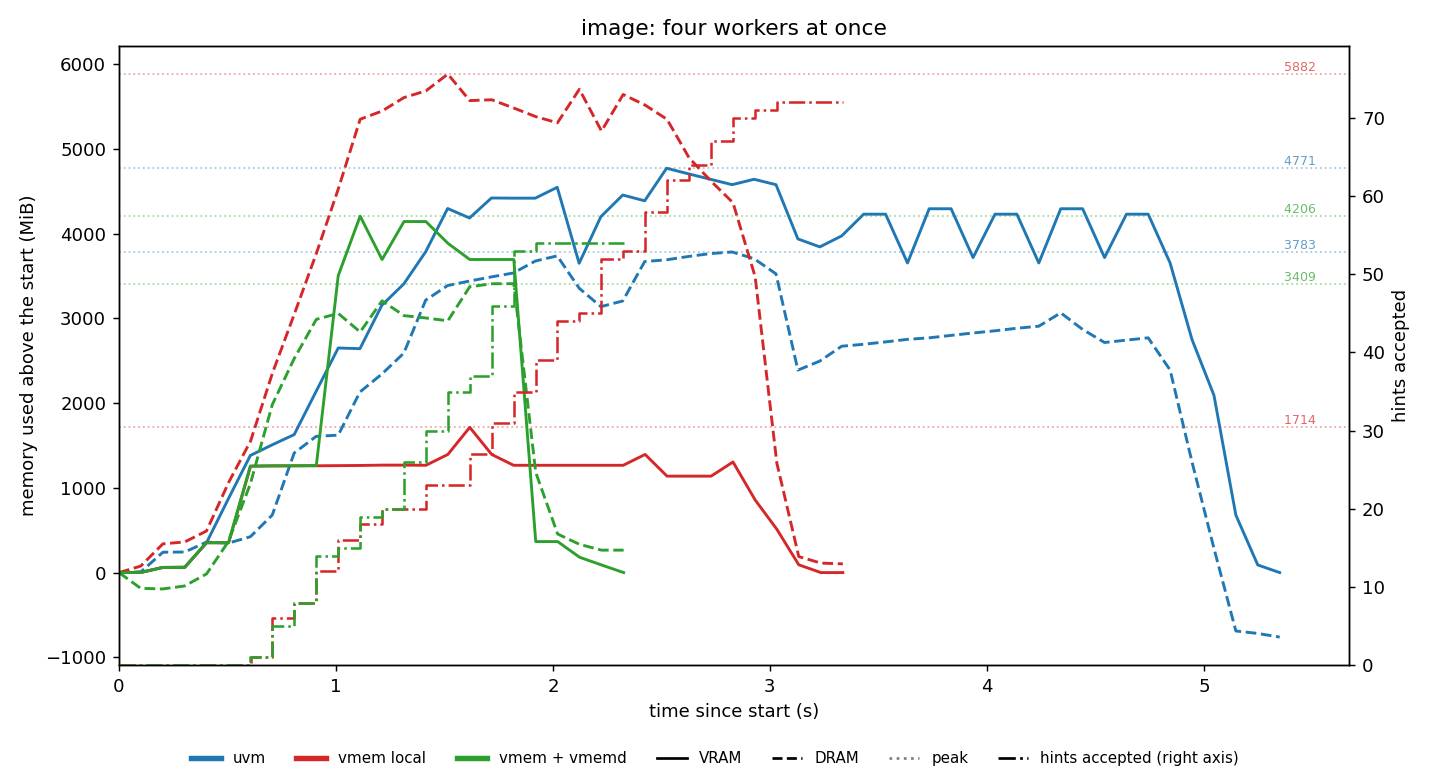
\includegraphics[width=\linewidth]{../libvmem/analysis/image.png}
\caption{Memory use over time in the image workload. VRAM (solid) and DRAM
(dashed) are shown above their values at the start. The right axis counts the
hints that moved data in each \code{vmem} run.}
\label{fig:lv-image}
\end{figure}

In our experiments we observed the following.

\begin{itemize}
  \item Every workload needs more than the VRAM, so \code{cuda} ran out of
    memory in all three. Every other configuration finished, and every
    process passed its result checks.
  \item In the image workload, both \code{vmem} configurations finished
    first. \code{vmem} + \vmemd took \SI{3.5}{\second}, against
    \SI{9.1}{\second} for \code{uvm}.
  \item Spilling costs pinned host memory, which the OS cannot swap out. In
    the image workload, \code{vmem} local pinned up to \SI{6825}{\mebi\byte}
    of DRAM (\cref{fig:lv-image}). The broker held it to
    \SI{3230}{\mebi\byte}.
  \item The broker reached its host limit and refused 30 evictions in the
    image workload. Those images stayed on the device, and 22 later
    prefetches found their image already there. Only 68 hints moved data,
    against 120 in \code{vmem} local. We think these saved copies make the
    broker run the faster of the two.
  \item In the GEMM workload, which gives no hints, all configurations took
    about \SI{16}{\second}. \code{vmem} placed the matrices that did not fit
    in host memory, and this cost no time here.
  \item In the mix workload, \code{vmem} took about \SI{6.5}{\second}, and
    \code{uvm} and \code{raw} took about \SI{11.3}{\second}. The hints did not
    help UVM in this workload. We have not found out why.
  \item In every run with \vmemd, the broker's counts returned to zero when
    the processes exited.
\end{itemize}

Each configuration ran once, on one GPU. \Cref{sec:limitations} lists the
limits of this setup.

\TODO{Rerun each configuration 5 times (tracker 1Biv), then replace the table with the median and range.}

\subsection{What the broker cannot see}
\label{sec:lv-gap}

The broker counts bytes, but it does not know which memory a kernel will use
next. It can refuse a move, but it cannot choose which buffer to evict,
because a general CUDA program never says which buffers its kernels touch.
The application must place every hint by hand, and each hint waits for the
whole process to go idle. A framework that knows which tensors each operation
reads and writes can supply this information. \Cref{sec:pytorch} describes
our plan to get it from PyTorch.
